

\section{Main Experiments}
Our model is a unified omni-modal system capable of processing text, vision, and speech simultaneously. Accordingly,
we compare against Qwen3-Omni-A3B-Instruct, the current state-of-the-art omni modal, as the primary baseline to
situate our model within the competitive landscape of full-modality systems. In addition, to rigorously assess the visual
understanding capability of our model in isolation, we further include Qwen3-VL-A3B, a dedicated vision-language
model optimized purely for visual comprehension, as a complementary reference. In the audio domain, we also compare with audio-specialized models including MiMo-Audio~\cite{zhang2025mimo}, Kimi-Audio~\cite{ding2025kimi}, and Step-Audio-2-mini~\cite{wu2025step}. We conduct a comprehensive evaluation across the following dimensions:






\subsection{Main Results}




\subsubsection{Visual Understanding}
\textbf{STEM.}

We conduct a comprehensive evaluation of our model across a diverse suite of multimodal reasoning benchmarks to rigorously assess its reasoning capabilities under complex logic. 
The evaluated datasets encompass multi-disciplinary queries (MMMU~\cite{yue2024mmmu}, MMMU-Pro~\cite{yue2025mmmu}) and mathematics-focused tasks (MathVista~\cite{lu2023mathvista}, MathVision~\cite{wang2024measuring}).
On mathematical reasoning benchmarks, our model demonstrates superior performance, achieving the highest scores among all compared models on MathVista (83.1) and MathVision (64.7). Notably, it outperforms specialist MLLMs such as InternVL3.5-A3B-Flash and Qwen3-VL-A3B-Instruct in these domains. In comprehensive multi-discipline evaluations, our model exhibits competitive performance; it surpasses Qwen3-Omni-A3B-Instruct on both MMMU (70.6) and MMMU-Pro (60.3).

We extend our evaluation to VisuLogic~\cite{DBLP:journals/corr/abs-2504-15279} and BabyVision~\cite{DBLP:journals/corr/abs-2601-06521}, which serve as rigorous testbeds for vision-centric reasoning. Although we did not specifically optimize towards these datasets, the empirical results are surprisingly strong. On the VisuLogic benchmark, our model secures the top position with a score of 29.4, surpassing baselines including InternVL3.5-A3B-Flash (28.4) and Gemini2.5-Flash-Lite (26.1). Similarly, on BabyVision, the model maintains a competitive score of 14.4, outperforming InternVL3.5-A3B-Flash and Qwen3-Omni-A3B-Instruct, while standing moderately behind Gemini2.5-Flash-Lite (19.6) and Qwen3-VL-A3B-Instruct (16.0). These unexpected gains suggest that our model develops robust, emergent generalization capabilities for decoding complex visual logic puzzles.


\textbf{OCR.} To comprehensively evaluate the model's capability in document understanding 
and information extraction across diverse document types, we conduct assessments on OCRBench~\cite{ocrbench}, OCRBenchV2~\cite{ocrbenchv2}, 
DocVQA~\cite{docvqa}, and OmniDocBench~\cite{omnidocbench}. OmniDocBench is a comprehensive and challenging benchmark encompassing a wide variety of document types — including academic papers, financial reports, and administrative forms. As shown in Table \ref{tab:academic_results}, LongCat-Next-A3B scores 0.152 on $\text{OmniDocBench}_{\text{en}}$ and 0.226 on $\text{OmniDocBench}_{\text{zh}}$, performing better than the other baselines listed and demonstrating that discrete modeling need not compromise fine-grained textual perception even under high-complexity, text-dense conditions. On the OCRBench benchmark, our model achieves a score of 865, outperforming baselines such as Qwen3-Omni-A3B-Instruct, GPT5-minimal, and Gemini2.5-Flash-Lite. 

Furthermore, to 
evaluate the model's ability to process structured visual information 
in charts and figures, we additionally benchmark on ChartQA~\cite{chartqa}, 
CharXiv~\cite{charxiv}, and InfoVQA~\cite{infovqa}. As shown in Table \ref{tab:academic_results}, our model achieves the best performance among all models  on $\text{CharXiv}_{\text{RQ}}$ and ChartQA, with scores of 60.1 and 88.0, respectively. On $\text{CharXiv}_{\text{DQ}}$, it obtains a score of 89.9, outperforming other baselines and ranking second only to Gemini2.5-Flash-Lite.



\begin{figure}[t]
    \centering
    \includegraphics[width=1.0\linewidth]{figs/case_und_gen.pdf}
    \caption{The understanding and generation cases of LongCat-Next at arbitrary resolution.}
    % \vspace{-4pt}
    \label{fig:case_und_gen}
\end{figure}



\paragraph{General Domains.} %MMBench, RealWorldQA, and MMStar.
We conduct a comprehensive evaluation across multiple mainstream benchmarks, such as MMBench~\cite{DBLP:conf/eccv/LiuDZLZZYWHLCL24}, RealWorldQA~\cite{realworldqa2024}, and MMStar~\cite{DBLP:conf/nips/ChenLDZZCDWQLZ24}, to systematically measure the general VQA capabilities. Across general-domain evaluations, our proposed model demonstrates highly competitive performance. On the MMStar benchmark, our model achieves a score of 69.3, outperforming baselines such as Qwen3-Omni-A3B-Instruct (68.5) and GPT5-minimal (65.2). Notably, it maintains performance levels that are closely comparable to specialist multimodal large language models (MLLMs), including Qwen3-VL-A3B-Instruct (72.1). Similarly, on RealWorldQA (72.0), our model yields robust results, successfully surpassing Gemini2.5-Flash-Lite (70.5). For CountBench, our model secures a commendable score of 82.5, performing comparably to Qwen3-Omni-A3B-Instruct (83.8), although it trails slightly behind the top-performing models in this specific category, such as Gemini2.5-Flash-Lite (90.0).


% \paragraph{Grounding.}

\paragraph{Graphical User Interface (GUI).}
We evaluate UI perception capabilities across diverse digital environments through GUI-grounding tasks like OSWorld-G~\cite{xie2025scalingcomputerusegroundinguser}, and ScreenSpot-V2~\cite{wu2024atlas}. Our model demonstrates highly competitive performance, maintaining parity with Qwen3-Omni-A3B-Instruct and Qwen3-VL-A3B-Instruct. This validates that our architecture effectively captures the visual granularity required for complex interfaces. While the current data mixture contains a limited proportion of high-resolution samples, optimizing for higher-density modeling remains a key objective for our next iteration.

\begin{table}[t]
\centering
\small 
\caption{Comparison of LongCat-Next and top-tier models on vision benchmarks. Values marked with * are sourced from public reports.}
\label{tab:academic_results}
\vspace{1em}
\setlength{\tabcolsep}{3pt}
\begin{tabularx}{\textwidth}{c*{7}{>{\raggedright\arraybackslash}X}}
\toprule
\multirow{3}{*}{\textbf{Benchmark}} & \multirow{3}{=}{\textbf{LongCat-Next}} & \multirow{3}{=}{\textbf{Qwen3-Omni-A3B-Instruct}} & \multirow{3}{=}{\textbf{GPT5-minimal}} & \multirow{3}{=}{\textbf{Gemini2.5-Flash-Lite}} & \multicolumn{2}{c}{\textbf{Specialist MLLMs}} \\
 \cmidrule(r){6-7}
  & &&&&\textbf{InternVL3.5-A3B-Flash} & \textbf{Qwen3-VL-A3B-Instruct}  \\
\midrule
\multicolumn{7}{c}{\textbf{STEM \& Reasoning}} \\
\midrule
MMMU-Pro & 60.3 & 57.0$^*$ &62.7$^*$ & 64.1 & -- & 60.4$^*$ \\ 
MMMU$_{\text{val}}$ & 70.6 & 69.1$^*$ &74.4$^*$ & 74.9 & 75.6$^*$ &  74.2$^*$ \\ 
MathVista$_{\text{mini}}$ & 83.1 & 75.9$^*$ & 50.9$^*$ & 78.2 &80.9$^*$& 80.1$^*$\\
MathVision & 64.7 & 56.3$^*$ & 45.8$^*$ & 61.9 &55.7$^*$& 60.2$^*$\\
VisuLogic & 29.4 & 20.0 & -- & 26.1 & 28.4 & 23.0$^*$  \\
BabyVision & 14.4 & 11.9 & -- & 19.6 & 11.3 & 16.0 \\
\midrule
\multicolumn{7}{c}{\textbf{OCR \& Doc \& Chart}} \\
\midrule
 OmniDocBench$_{\text{en}}$ $\downarrow$ & 0.152 & 0.289 & 0.174$^*$ & 0.240 & 0.246 & 0.183$^*$\\
OmniDocBench$_{\text{zh}}$ $\downarrow$ & 0.226 & 0.406 & 0.389$^*$ & 0.312 &  0.359 & 0.253$^*$ \\
CharXiv$_{\text{DQ}}$ & 89.9 & 78.8 & 79.5$^*$ & 91.2 & 81.8$^*$ & 85.5$^*$ \\
CharXiv$_{\text{RQ}}$ & 60.1 & 42.8 & 57.8$^*$ & 60.0 & 48.0$^*$ & 48.9$^*$ \\
ChartQA & 88.0 & 86.8$^*$ & 59.1$^*$ & 79.0 & 87.4$^*$ & 86.8$^*$\\
InfoVQA$_{\text{test}}$ & 83.3 & 84.4 & 69.9$^*$ & 82.2 & 81.4$^*$& 81.8$^*$\\
DocVQA$_{\text{test}}$ & 94.2 & 94.1 & 89.6$^*$ & 91.8 & 94.2$^*$ & 95.0$^*$\\
OCRBench & 86.5 & 85.4$^*$ & 78.7$^*$ & 84.8 & 88.0$^*$ & 90.3$^*$ \\
OCRBenchV2$_{\text{en}}$ & 58.5 & 62.0 & 48.2$^*$ & 51.5 & 47.0 & 63.2$^*$ \\
OCRBenchV2$_{\text{zh}}$ & 59.3 & 60.5 & 37.7$^*$ & 39.5 & 48.2 & 57.8$^*$ \\
\midrule
\multicolumn{7}{c}{\textbf{Agent}} \\
\midrule
OSWorld-G & 58.3 & 60.3 & -- & -- & 42.4$^*$ & 60.5$^*$ \\
ScreenSpot-V2 & 88.3 & 91.8 & -- & -- & 87.3$^*$ & 87.7 \\
\midrule
\multicolumn{7}{c}{\textbf{General}} \\
\midrule
MMStar & 69.3 & 68.5$^*$ & 65.2$^*$ & 74.93 & 72.0 & 72.1\\
RealWorldQA & 72.0 & 72.9 & 77.3$^*$ & 70.5 & 72.3 & 73.7\\
CountBench & 82.1 & 83.8 & 87.8$^*$ & 90.0 & 84.2 & 90.6\\

\bottomrule
\end{tabularx}

\end{table}



\subsubsection{Visual Generation}

We evaluate our model's text-to-image (T2I) capability across a diverse set of public benchmarks, covering compositional reasoning, prompt fidelity, long-text understanding, world knowledge, and text rendering.
We evaluate on GenEval \cite{ghosh2023genevalobjectfocusedframeworkevaluating} (compositional alignment), DPG-Bench \cite{hu2024ella} (prompt following),  WISE \cite{niu2025wise} (world knowledge and reasoning), and LongText-Bench \cite{geng2025xomni} / TIFF \cite{wei2025tiif} / CVTG-2K\cite{du2025textcrafter} (text rendering).
Baselines are grouped into (i) unified multimodal models and (ii) specialized T2I models.


\begin{table}[t]
\centering
\caption{Comparison with specialized T2I models. Despite significantly smaller model, our model achieves competitive performance across multiple benchmarks, demonstrating strong industrial-level generation capability. Values marked with * are sourced from public reports.}
\vspace{1em}
\label{tab:t2i_specialized}
\resizebox{1.0\textwidth}{!}{
\begin{tabular}{lllllllll}
\toprule
\textbf{Model} & \multicolumn{1}{c}{\textbf{GenEval}} & \multicolumn{1}{c}{\textbf{DPG}} & \multicolumn{1}{c}{\textbf{LongText-EN}} & \multicolumn{1}{c}{\textbf{LongText-ZH}} & \multicolumn{1}{c}{\textbf{WISE}} & \multicolumn{1}{c}{\textbf{TIFF}} & \multicolumn{1}{c}{\textbf{CVTG}}  \\
\midrule
Emu-3.5 \cite{cui2025emu3}              & 72.67 & ${89.42}^{*}$ & ${97.60}^{*}$ & ${92.80}^{*}$ & 57.64 & ${89.48 / 88.18}^{*}$ & ${91.23}^{*}$ \\

Qwen-Image 2507  \cite{wu2025qwenimagetechnicalreport}      & ${87.00}^{*}$ & ${88.32}^{*}$ & ${94.30}^{*}$ & ${94.60}^{*}$ & ${63.00}^{*}$ & ${86.10}^{*}$ / ${86.80}^{*}$ & ${82.88}^{*}$ \\
Gemini 2.5 Flash Image \cite{comanici2025gemini25pushingfrontier} & 79.67 & 85.82 & 86.04 & - & 76.27  & 90.53 / 90.80 & ${73.64}^{*}$ \\
FLUX.1-dev  \cite{labs2025flux1dev}        & ${66.00}^{*}$ & ${84.00}^{*}$ & ${60.70}^{*}$ & ${0.50}^{*}$  & ${50.00}^{*}$ & ${71.10 / 71.80}^{*}$ & ${49.65}^{*}$ \\
Seeddream 3.0  \cite{gao2025seedream} & - & ${94.31}^{*}$ & ${89.60}^{*}$ & ${87.80}^{*}$  & - & ${86.02 / 84.31}^{*}$ & ${59.24}^{*}$ \\

\midrule
LongCat-Next  & 84.44 & 84.66 & 93.15 & 89.08 & 57.00 & 82.85  / 84.38 & 76.36 \\
\bottomrule
\end{tabular}
}
\end{table}

\paragraph{Analysis of Results.} \textbf{(1) Clear Advantage over Unified Multimodal Models.}
Our model outperforms prior unified approaches across most benchmarks, establishing a new performance level for generation within unified architectures. The gains are particularly significant on long-text understanding and text rendering (LongText, TIFF, CVTG-2K), where our model shows clear margins over existing methods.
We attribute this improvement to our \textbf{Unified architecture}, which tightly integrates language understanding with image generation. By enabling stronger semantic planning before synthesis, the model better preserves textual intent in complex scenarios such as multi-object composition and text rendering, where prior unified models often struggle. \textbf{(2) Competitive Performance with Specialized T2I Models.}
Despite being a unified model, our approach achieves competitive performance compared to specialized T2I systems. Notably, it matches or exceeds larger models on GenEval and LongText-Bench, and remains competitive on text rendering benchmarks.
This suggests that strong generation capability can be achieved without dedicated task-specific architectures, and that integrating understanding and generation can provide complementary benefits beyond pure scaling. Overall, our results indicate that unified multimodal models can surpass prior limitations in generation quality when equipped with stronger language-guided generation mechanisms. This enables a favorable balance between capability, efficiency, and deployment practicality.



\begin{table*}[t]
\centering
\small
\caption{Comparison with unified multimodal models. We evaluate across both understanding and generation benchmarks. Our model (LongCat-Next) consistently outperforms prior unified approaches across most generation benchmarks while maintaining highly competitive understanding capabilities, establishing a new state-of-the-art for unified generation-understanding models. All results are from public reports.}
\label{tab:omni_unified_results}
\vspace{1em}
\resizebox{\textwidth}{!}{
\begin{tabular}{l ccccc | cccccc}
\toprule
\multirow{2}{*}{\textbf{Model}} & \multicolumn{5}{c|}{\textbf{Understanding}} & \multicolumn{6}{c}{\textbf{Generation}} \\
\cmidrule(lr){2-6} \cmidrule(lr){7-12}
& \textbf{MMMU} & \textbf{MathVista} & \textbf{OCRBench}  & \textbf{DocVQA} & \textbf{MMStar} & \textbf{GenEval} & \textbf{DPG} & \textbf{LT-EN/ZH} & \textbf{WISE} & \textbf{TIFF} & \textbf{CVTG} \\
\midrule
Janus-Pro \cite{chen2025janus} & 41.0 & -- & -- & -- & -- & 80 & 84.19 & 1.90 / 0.60 & 35 & 65.50 / 68.80 & -- \\
Show-o2\cite{xie2025showo2improvednativeunified}  & 48.9 & -- & --  & -- & 56.6 & 76 & 86.14 & -- / -- & -- & 65.80 / 65.00 & -- \\
OneCAT \cite{li2025onecatdecoderonlyautoregressivemodel} & 41.9 & 61.7 & --  & 91.2 & -- & 90 & 84.53 & -- / -- & -- & -- & -- \\
Mogao \cite{liao2025mogaoomnifoundationmodel} & 44.2 & --  & -- & -- & -- & 89 & 84.33 & -- / -- & -- & -- & -- \\
BAGEL \cite{deng2025emergingpropertiesunifiedmultimodal} & 55.3 & 73.1 & 80.9  & 92.2 & 69.3 & 82 & 85.07 & 43.70 & 4.70 / 49 & 71.50 / 71.70 & 35.60 \\
NEO-unify \cite{diao2026pixelswordsnative} & 68.9 & -- & 81.5  & 91.6 & 65.5 & 85 & 86.71 & 91.40 / 75.50 & 42 & -- & -- \\
Ovis-U1\cite{wang2025ovisu1technicalreport} & 51.1 & 69.4 & 88.3  & -- & -- & 89 & 83.72 & 3.00 / 5.10 & 42 & 66.70 / 68.20 & 9.30 \\
Lumina\cite{xin2025luminadimooomnidiffusionlarge} & 58.6 & -- & -- & --  & -- & 88 & 86.04 & 43.70 / 4.70 & 40 & 74.70 / 72.00 & 59.00 \\
OmniGen2\cite{wu2025omnigen2explorationadvancedmultimodal} & 53.1 & -- & -- & --  & -- & 80 & 83.57 & 56.10 / 5.90 & -- & -- & -- \\
UniWorld-V1\cite{lin2025uniworldv1highresolutionsemanticencoders} &  58.6 & -- & --  & -- & -- & 80 & 81.38 & -- / -- & 55 & -- & -- \\
X-Omni \cite{geng2025xomni}& -- & -- & 70.4  & -- & -- & 83 & 87.65 & 90.00 / 81.40 & -- & -- & -- \\
InternVL-U\cite{tian2026internvludemocratizingunifiedmultimodal} & 54.7  & -- & 83.9 & -- & --  & 85 & 85.18 & 73.80 / 86.00 & 46 & 74.90 / 73.90 & 62.30 \\
BLIP3-o \cite{blip3oNext2025} & 50.6   & -- & -- & -- & -- & 84 & 81.60 & -- / -- & 62 & -- & -- \\
\midrule
LongCat-Next & 70.6 & 83.1 & 86.5  & 94.2 & 69.3 & 84 & 84.66 & 93.15 / 89.08 & 57 & 82.85  / 84.38 & 76.36  \\
\bottomrule
\end{tabular}
}
\end{table*}



\subsubsection{Audio}

We conduct a comprehensive evaluation of the audio capability of LongCat-Next, covering automatic speech recognition (ASR), text-to-speech (TTS), audio understanding, and audio-to-text chat.
ASR and TTS serve as foundational tasks for evaluating speech understanding and generation. To assess ASR performance, we utilize a range of benchmark datasets, including LibriSpeech~\cite{panayotov2015librispeech}, AISHELL-1~\cite{bu2017aishell}, AISHELL-2~\cite{du2018aishell}, FLEURS~\cite{conneau2023fleurs}, and WenetSpeech~\cite{zhang2022wenetspeech}. Meanwhile, for evaluation of TTS, both the Chinese and English versions of SeedTTS~\cite{anastassiou2024seed} are used to ensure comprehensive coverage. For ASR and TTS task, we report the WER metric for evaluation.
Beyond these tasks, audio understanding focuses on the model’s ability to perceive and reason about fine-grained acoustic information within input audio, such as speech, environmental sounds, music, speaker gender, age, accent, etc. Consequently, we adopt MMAU~\cite{sakshi2024mmau}~\footnote{MMAU v05.15.25 test-mini}, VocalSound~\cite{gong2022vocalsound}, TUT2017~\cite{mesaros2016tut},  and ClothoAQA~\cite{lipping2022clotho}as standard benchmarks for this purpose. Furthermore, to measure LongCat-Next’s performance in audio-instructed conversations, OpenAudioBench~\cite{li2025baichuan} is used as the evaluation benchmark, examining the model’s capabilities in world knowledge, mathematical proficiency, and reasoning ability. To ensure standardized and reproducible results, we employ the evaluation method released by Kimi-Audio-Evalkit~\footnote{\url{https://github.com/MoonshotAI/Kimi-Audio-Evalkit}}. We use \textit{gpt-4o-2024-08-06} as the judge model for tasks like audio question answering. Through multi-faceted evaluation approaches, we provide a thorough assessment of the model’s performance across diverse audio tasks.

\begin{table}[t]
\centering
\footnotesize
\setlength{\tabcolsep}{2pt}
\renewcommand{\arraystretch}{0.9}
\caption{Comparison of LongCat-Next and top-tier models on audio benchmarks.Values marked with * are sourced from public reports.}
\vspace{1em}
\label{tab:audio_res}
\begin{tabularx}{\textwidth}{l*{7}{>{\centering\arraybackslash}X}}
\toprule
\multirow{3}{*}{\textbf{Benchmark}} & \textbf{LongCat-Next} & \textbf{Gemini-3.1-Flash-Lite-preview} & \textbf{Gemini-2.5-Flash-Lite-preview} & \textbf{Qwen3-Omni-A3B-Instruct} & \textbf{MiMo-Audio} & \textbf{Kimi-Audio} & \textbf{Step-Audio-2-mini}\\
\midrule
\multicolumn{8}{c}{\textbf{ASR}} \\
\midrule
% \makecell[l]{LibriSpeech \\ \footnotesize test-clean | test-other} & 1.63 | 3.42 & 2.39 | 5.79 & 3.14 | 7.25 & 1.22 | 2.48 & 3.76 | 21.59 & 1.28 | 2.42 & 1.33 | 2.86  \\
LibriSpeech$_\text{test-clean}$ $\downarrow$ &1.63&2.38&3.14&1.22$^*$&2.47&1.28$^*$&1.33$^*$ \\
LibriSpeech$_\text{test-other}$ $\downarrow$ &3.42&5.68&7.19&2.48$^*$&6.13&2.42$^*$& 2.86$^*$\\
AISHELL-1  $\downarrow$  & 1.47 & 6.00 & 11.64 &  0.84$^*$ & 1.69 & 0.60$^*$ & 0.78$^*$ \\
AISHELL-2  $\downarrow$     & 2.82 & 8.00 & 15.33 & 2.34$^*$ & 3.02 & 2.56$^*$ & 2.16$^*$ \\

Fleurs$_\text{zh}$ $\downarrow$ &3.24&3.88&7.77&2.20$^*$&9.29&2.69$^*$&2.53$^*$ \\
Fleurs$_\text{en}$ $\downarrow$ &5.24&5.96&6.84&2.72$^*$&6.33&4.44$^*$& 3.05$^*$\\

WenetSpeech$_\text{test-meeting}$ $\downarrow$ &8.19 &20.37 &23.04&5.89$^*$&9.49&6.28$^*$& 4.87$^*$\\
WenetSpeech$_\text{test-net}$ $\downarrow$ &5.98&16.15&24.83&4.69$^*$&7.64&5.37$^*$&4.82$^*$ \\
\midrule
\multicolumn{8}{c}{\textbf{TTS}} \\
\midrule

SeedTTS$_\text{zh}$ $\downarrow$& 1.90 & - & - & 1.07$^*$ & 1.96$^*$ & 13.46 & 2.13$^*$ \\
SeedTTS$_\text{en}$ $\downarrow$& 1.89 & - & - & 1.39$^*$ & 5.37$^*$ & 29.45 & 3.18$^*$ \\
\midrule


\multicolumn{8}{c}{\textbf{Audio Understanding}} \\
\midrule
MMAU         & 76.40 & 71.70 & 74.80 & 78.20 & 75.80 & 70.31 & 71.30 \\
ClothoAQA    & 73.45 & 60.53 & 63.27 & 75.16$^*$ & 68.85 & 72.21$^*$ & 68.39$^*$ \\
TUT2017      & 43.09 & 23.15 & 22.47 & 40.74$^*$ & 15.06 & 65.25$^*$ & 30.67$^*$ \\
VocalSound   & 85.91 & 69.81 & 57.67 & 91.59$^*$ & 87.94 & 94.85$^*$ & 87.58$^*$ \\
\midrule
\multicolumn{8}{c}{\textbf{Audio-to-Text Chat}} \\
\midrule
AlpacaEval     & 86.83 & 62.56 & 89.05 & 90.10 & 85.67 & 78.74 & 53.06 \\
LlamaQuestions & 79.67 & 82.67 & 83.33 & 82.33 & 75.00 & 79.33 & 69.70 \\
ReasoningQA    & 87.52 & 65.64 & 74.06 & 87.62 & 75.34 & 68.61 & 63.86 \\
TriviaQA       & 67.60 & 68.40 & 66.90 & 76.60 & 50.30 & 62.10 & 45.30\\
Webquestions   & 69.10 & 69.10 & 70.00 & 75.90 & 61.30 & 70.30 & 56.90 \\
\bottomrule
\end{tabularx}
\end{table}

Table~\ref{tab:audio_res} summarizes the evaluation results of audio capabilities in comparison with other competitors, including Gemini-3.1-Flash-Lite-preview, Gemini-2.5-Flash-Lite-preview~\cite{comanici2025gemini25pushingfrontier}, Qwen3-Omni-A3B-Instruct~\cite{xu2025qwen3}, MiMo-Audio~\cite{zhang2025mimo}, Kimi-Audio~\cite{ding2025kimi}, and Step-Audio-2-mini~\cite{wu2025step}. LongCat-Next demonstrates impressive fundamental audio capabilities, excelling at both audio recognition and synthesis. Notably, its performance in text-to-speech synthesis surpasses most compared models in terms of accuracy. Moreover, LongCat-Next achieves state-of-the-art performance across a wide range of audio comprehension tasks. These findings suggest that LongCat-Next possesses advanced capabilities in processing and understanding both general and complex acoustic information, far surpassing traditional speech recognition systems. Additionally, LongCat-Next shows strong results on audio-instructed question-answering benchmarks, highlighting its extensive world knowledge and advanced reasoning abilities.


\subsubsection{Text}
\begin{table}[t]
    \centering
    \small
    \caption{Comparison between \longcat and other models. Values marked with * are sourced from public reports.}
    \label{tab:chat_model_results}
    \vspace{1em}
    \begin{tabularx}{\textwidth}{l c*{5}{>{\raggedright\arraybackslash}X}}
    \toprule
    \multirow{2}{*}{\textbf{Benchmark}} & \textbf{\longcat} & \textbf{Kimi-Linear-48B-A3B} & \textbf{Qwen3-Next-80B-A3B-Instruct} & \textbf{Qwen3-Omni-A3B-Instruct} \\
        \midrule
        \multicolumn{5}{c}{\textbf{Agentic Tool Use}} \\
        \midrule
        Tau2-Airline(avg@8) & {56.50}& 44.00 & 45.5* & 27.00  \\
        Tau2-Retail(avg@8) & {73.68}& 18.86 & 57.3* & 40.80  \\
        Tau2-Telecom(avg@8) & {62.06} & 15.68 & 13.2* & 4.39  \\
        VitaBench(avg@4) & {5.80} & - & {5.80} & - \\
        \midrule
        \multicolumn{5}{c}{\textbf{Agentic Coding}} \\
        \midrule
        SWE-Bench(acc) & {43.00} & 32.80 & 37.60 & - \\
        TerminalBench(acc) & {18.75} & {20.00} & 15.19 & - \\
        \midrule
        \multicolumn{5}{c}{\textbf{General Domains}} \\
        \midrule
        MMLU(acc) & 83.95 & 79.91 & {89.28} & 87.10 \\
        MMLU-Pro(acc) & 77.02 & 67.22 & {82.93} & 79.89 \\
        CEval(acc) & 86.80 & 78.48 & {90.91} & 88.50   \\
        CMMLU(acc) & 82.13 & 76.26 & {86.50} & 85.76   \\
        \bottomrule
    \end{tabularx}
    
\end{table}

Table~\ref{tab:chat_model_results} presents the foundational text-modality evaluation of \longcat. To comprehensively assess its pure-language cognitive abilities—which are crucial for supporting complex cross-modal reasoning—our evaluation framework is structured around three pivotal dimensions: agentic tool use, coding capabilities, and general-domain knowledge. The results demonstrate that \longcat establishes a formidable baseline, particularly excelling in practical execution. \textbf{(1) Excellence in Agentic Workflows and Coding.} We measure the model's capacity for environmental interaction and complex software engineering via Vita Bench~\cite{he2025vitabench}, a curated noise-reduced $\tau^2$-Bench\footnote{\url{https://github.com/AGI-Eval-Official/tau2-bench-revised}}, SWE-Bench~\cite{jimenez2023swe}, and TerminalBench~\cite{merrill2026terminalbenchbenchmarkingagentshard}. \longcat exhibits a distinct and overwhelming advantage in these scenarios. In tool-use evaluations, it establishes a clear lead across all $\tau^2$-Bench sub-scenarios, most notably achieving an exceptional 62.06 in the Telecom domain, completely eclipsing Qwen3-Omni-A3B-Instruct (4.39) and Kimi-Linear-48B (15.68). This proficiency extends to coding, where it achieves a 43.0 accuracy on the highly challenging SWE-Bench, significantly outperforming both Kimi-Linear-48B and Qwen3-Next. These results underscore its superior capability in dynamic environment navigation, complex tool dependency resolution, and real-world codebase manipulation. \textbf{(2)Robust Foundational Knowledge and Reasoning.} Beyond execution, \longcat successfully mitigates the ``multimodal tax''—a common performance degradation in text capabilities when scaling non-linguistic modalities. Broad multi-disciplinary knowledge and reasoning are tested across standard encyclopedic and mathematical benchmarks, including MMLU~\cite{hendrycks2021measuringmassivemultitasklanguage}, MMLU-Pro~\cite{wang2024mmluprorobustchallengingmultitask}, C-Eval~\cite{huang2023ceval}, CMMLU~\cite{li2023cmmlu}. \longcat consistently outperforms Kimi-Linear-48B and remains highly competitive with the multimodal Qwen3-Omni-A3B-Instruct. While the strictly text-optimized Qwen3-Next-80B-Instruct naturally sets the upper bound in these traditional academic tests, \longcat maintains a highly resilient cognitive baseline, ensuring its multimodal outputs are anchored by deep logical reasoning.



\subsection{Experimental Analysis of Methodology}
\label{sec:model_analysis}

We conduct ablation studies to analyze the key components of our method and the motivations behind their design. Due to the computational cost of full-scale experiments, some studies are conducted under a reduced setting using Qwen-7B as the language backbone. The detailed experiments are described below.

\subsubsection{Bridging the Understanding Gap Between Discrete and Continuous Modeling}


\begin{figure}[t]
     \centering
    % 左侧 minipage 放图片
    \begin{minipage}[c]{0.38\textwidth}
        \centering
        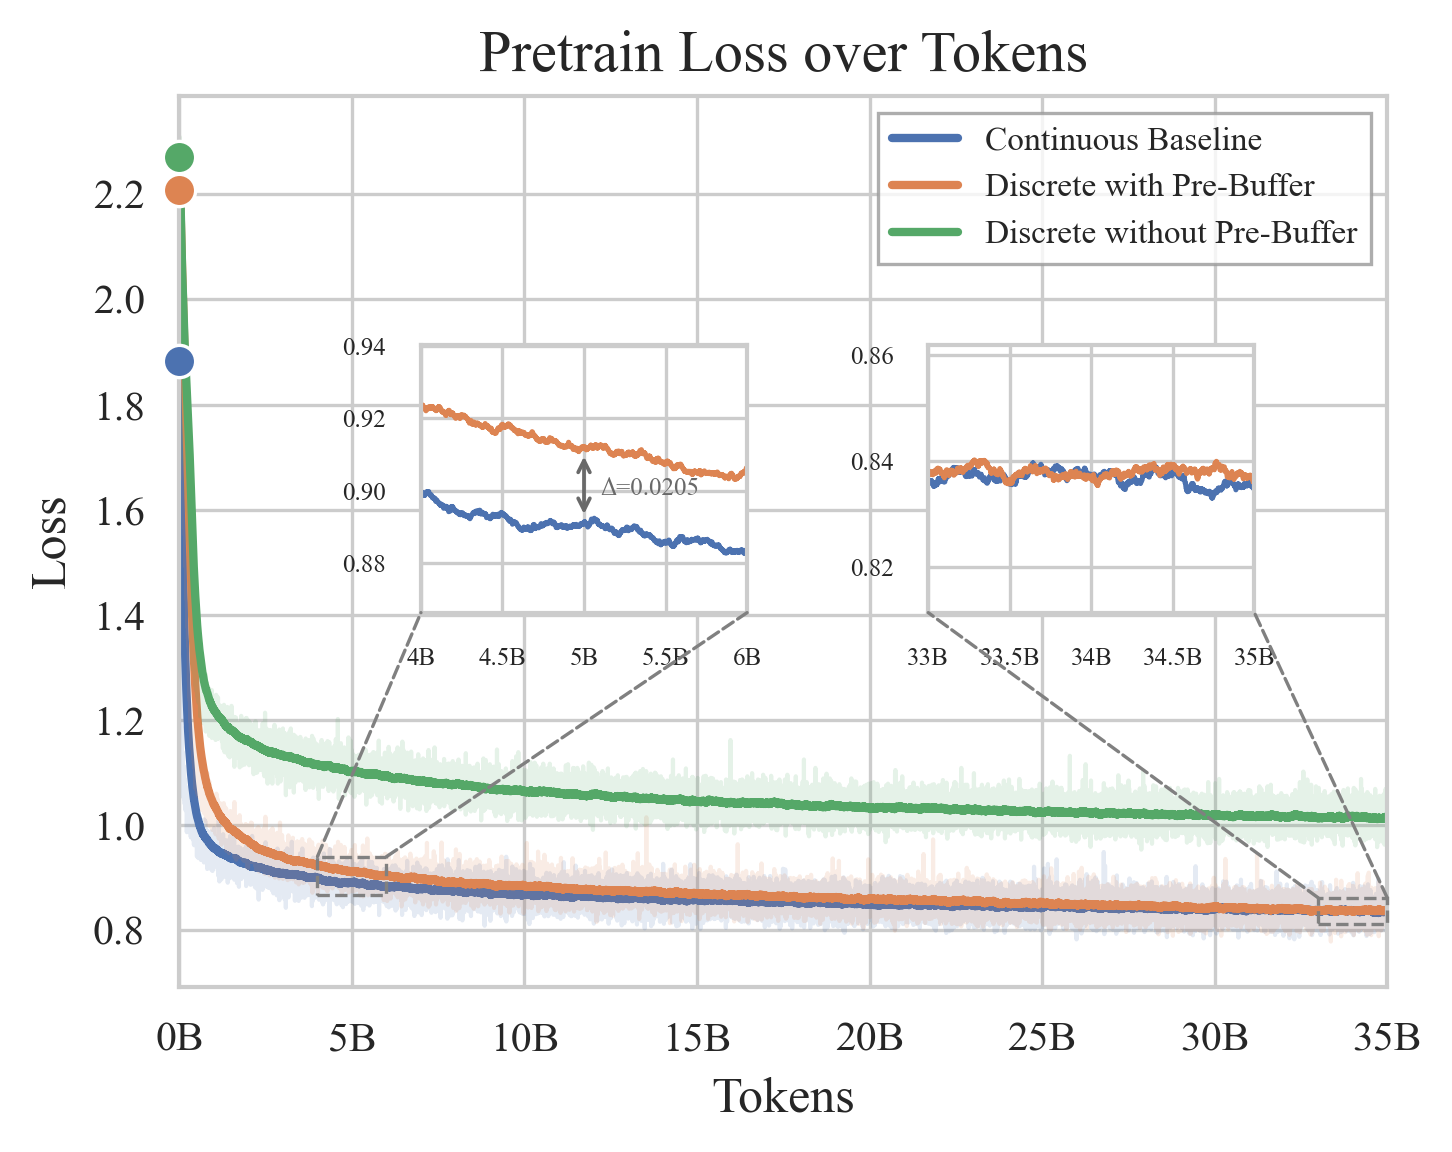
\includegraphics[width=\linewidth]{figs/discrete_loss.png}
    \end{minipage}
    \hfill
    % 右侧 minipage 放表格
    \begin{minipage}[c]{0.6\textwidth}
        \centering
        \scriptsize
        \renewcommand{\arraystretch}{1.0}
        \setlength{\tabcolsep}{3pt}
        \begin{tabular}{l|ccccc|cc}
        \toprule
        & \multicolumn{5}{c|}{\textbf{Partial Data}} & \multicolumn{2}{c}{\textbf{Scale Up Data}} \\
        \midrule
        \textbf{Experiment ID} & \textbf{I} & \textbf{II} & \textbf{III} & \textbf{IV} & \textbf{V} & \textbf{VI} & \textbf{VII} \\
        \midrule
        Rep. Type & Continuous & Discrete & Continuous & Discrete & Discrete & Continuous & Discrete \\
        PT Tokens & 0.1B & 0.1B & 5B & 5B & 5B & 5B & 5B \\
        MT\&SFT Tokens & 4B & 4B & 4B & 4B & 4B & 300B & 300B \\
        Pre-Buffer & - & \cmark & - & \cmark & \xmark & - & \cmark \\
        \midrule
        \multicolumn{8}{c}{\textbf{OCR \& Doc \& Chart}} \\
        \midrule
        OCRBench & 779 & 598 & 776 & 720 & 705 & 858 & 844\\
        DocVQA & 88.2 & 78.0 & 88.9 & 86.7 & 85.2 & 96.0 & 96.0 \\
        % InfoVQA & 68.2 & 50.8 & 70.2 & 66.4 & 61.8 & 86.0 & 82.9 \\
        ChartQA & 80.1 & 71.6 & 80.6 & 76.8 & 75.4 & 84.0 & 84.0 \\
        \midrule
        \multicolumn{8}{c}{\textbf{STEM \& Reasoning}} \\
        \midrule
        MMMU$_{\text{val}}$ & 49.8 & 44.8 & 49.1 & 48.0 & 49.8 & 58.0 & 60.0 \\
        MathVista & 59.6 & 47.3 & 56.1 & 54.2 & 56.7 & 75.0 & 74.0 \\
        \bottomrule
        \end{tabular}
    \end{minipage}
    \vspace{1em}
    \caption{L: Loss comparison on pre-align stage. R: Performance comparison of discrete and continuous versions.}
    \label{fig_tab:combined_optimized_layout}
    \vspace{-5pt}
\end{figure}

\textbf{Modeling Analysis.} As discussed in Sec.\ref{sec:visual_tokenizer}, the SAE coupled with RVQ formulation effectively addresses the challenge of semantic completeness. Building upon this foundation, we further investigate the extent to which discrete representations can approximate their continuous counterparts, and accordingly design a pre-alignment experiment. In this setting, all modules, except for the frozen language backbone and vision encoders (i.e., discrete dNaViT vs.\ continuous NaViT), are optimized. During this stage, we employ a captioning loss as a proxy to quantify the information loss introduced by discretization relative to the continuous version.

As depicted in Fig. \ref{fig_tab:combined_optimized_layout}, our empirical analysis yields three key insights: 
(1) the initial training loss is significantly higher than that of the continuous baseline. This indicates that continuous features are inherently easier to align at the early stage. Although the gap narrows as training progresses, a noticeable performance discrepancy (Exp I and II) remains under the vanilla discrete formulation. 
(2) Pre-Buffer. We hypothesize that this gap stems from insufficient re-encoding after the sum-up operation on multi-level embeddings. To address this, we introduce a lightweight \textit{Pre-Buffer} module (implemented as a single-layer FFN) to remaps the visual representations after codebook lookup and re-encodes the multi-level summed features. Despite its simplicity, this module substantially accelerates convergence and improves the expressiveness of the discrete tokens.
(3) Longer-Training. Unlike the continuous setting, discrete visual embeddings are learned entirely from scratch. As a result, they require more data to reach comparable performance. Comparisons across experiments (e.g., Exp I vs. II and Exp IV vs. VII) show that the performance gap can be largely reduced through extended training and increased data scale.

\textbf{Closing the Understanding Gap with Continuous Models.} Tab. \ref{fig_tab:combined_optimized_layout} reveals that dNaViT not only achieves comparable training loss but also maintains downstream performance within approximately a 1\% margin of the continuous baseline. Although the discrete model initially underperforms under limited training data, scaling the data progressively closes this gap, with its loss asymptotically approaching that of the continuous counterpart. For instance, Exp VI and VII demonstrate that the discrete formulation achieves near-parity with the continuous model. This conclusion is further supported by large-scale experiments on LongCat-Next, which achieve performance competitive with specialized continuous models such as Qwen3-VL-A3B-Instruct. These results indicate that discrete modeling does not have an inherent performance ceiling. Instead, its performance is primarily influenced by the training data. With the appropriate data scaling and improved quality, the full potential of discrete representations can be unlocked.



\subsubsection{Information Recovery Analysis} 
\label{information_recovery}



We provide a previously underexplored perspective: the reconstruction capability of semantic encoders is not solely determined by supervision, but is also intrinsically linked to architectural properties such as residual connections. As evidenced in Fig.~\ref{fig:reconstruction_visuals} and Tab.~\ref{tab:reconstruction_metrics}, all decoders are paired with a lightweight ViT-based decoder to isolate encoder characteristics. Semantic encoders with residual pathways exhibit non-trivial reconstruction capability despite the absence of explicit reconstruction supervision (e.g., ResNet50). In contrast, QwenViT without the merger module achieves comparable reconstruction performance, while introducing the merger leads to noticeable degradation due to the aggressive downsampling ($14\times \rightarrow 28\times$), as shown in Fig.~\ref{fig:reconstruction_visuals}. Qualitative visualizations further suggest that such SAE-style encoders (e.g., QwenViT) still retain the ability to recover coarse image-level structures, but are only less effective at reconstructing fine-grained, high-frequency details. This provides an insightful perspective for rethinking the trade-off between pixel-level and semantic-level information.


\begin{table}[htbp]
    \centering
    \footnotesize % 学术报告建议字号
    \caption{Quantitative reconstruction performance across various visual encoder architectures. PSNR and SSIM represent reconstruction fidelity ($\uparrow$), while rFID measures perceptual discrepancy ($\downarrow$).}
    \vspace{1em}
    \label{tab:reconstruction_metrics}
    \setlength{\tabcolsep}{6pt} % 列间距（默认6pt，缩小一点）
    \renewcommand{\arraystretch}{1.05} % 行距更紧凑
    \begin{tabular}{l cccc}
        \toprule
        \textbf{Metric} & ResNet50 & {ViT-B/16 (Pretrained)} & {ViT-B/16 (Random)} & {QwenViT (w/o merger)}  \\
        \midrule
        PSNR ($\uparrow$) & $20.88 \pm 3.44$ & $21.86 \pm 3.14$ & $30.52 \pm 3.42$ & $18.16 \pm 2.61$ \\
        
        SSIM ($\uparrow$) & $0.509 \pm 0.174$ & $0.581 \pm 0.139$ & $0.887 \pm 0.051$ & $0.46 \pm 0.14$  \\
        
        rFID ($\downarrow$) & 0.4619 & 0.8850 & 0.5847 & 0.987 \\

        \bottomrule
    \end{tabular}
\end{table}




Interestingly, the vanilla ViT with randomly initialized weights achieves the best reconstruction performance, yielding the highest PSNR among the compared models. A possible explanation is that the outputs of a randomly initialized ViT tend to resemble noise-like signals, which are easier for the decoder to denoise during reconstruction. Meanwhile, the residual pathways in the architecture may still preserve a portion of the original pixel-level information.


\begin{figure}[h]
    \centering
    \includegraphics[width=1.0\linewidth]{figs/conflict_trainingloss.pdf}
    \caption{Visual understanding and generation interaction under DiNA framework.}
    \label{fig:und_and_gen}
\end{figure}

\subsubsection{Conflict between Understanding and Genearation}

Given that DiNA integrates understanding and generation through a unified autoregressive objective, we designed a set of illuminating experiments to investigate the conflicting or synergistic relationship between these two tasks. All training was conducted under identical experimental settings using the same model checkpoint. Specifically, we trained Pure-Und. and Pure-Gen. models using 100B tokens of understanding and generation data, respectively. Additionally, we trained a Unified model on a 1:1 mixture comprising 50B tokens from each dataset. Since the Unified model receives only half the task-specific data compared to the pure models under the same token budget, we proportionally scale its loss curve while retaining the original unscaled version for reference. Fig.~\ref{fig:und_and_gen} demonstrates that under comparable token counts, the Unified model exhibits a marginal loss difference of 0.006 compared to the Pure-Und. model, while achieving a loss of 0.02 lower than that of the Pure-Gen. model. This suggests that generation does not compromise understanding, whereas understanding actively enhances generation.

\subsubsection{Semantic Comparison of Parallel and Serial Audio Generation}
In parallel internal text-guided generation, each decoding step simultaneously generates both text and audio outputs. This mixed multimodal representation introduces considerable challenges in achieving semantically accurate responses.  In contrast, serial generation avoids this issue, inherently offering stronger semantic consistency by sequentially generating outputs.
To this end, we propose a random delay-based unified modeling paradigm for internal language guidance. Leveraging this approach, LongCat-Next adaptively learns to align audio and text semantics within the context, significantly reducing discrepancies between the two generation strategies.


To validate the effectiveness of our method, we systematically evaluate the text guidance accuracy on the LlamaQuestions and ReasoningQA benchmarks in an audio-to-audio manner. The results show that parallel generation achieves performance comparable to serial generation, with 79.33 vs. 81.67 on LlamaQuestions and 74.95 vs. 80.30 on ReasoningQA. Despite a slight gap, the parallel approach maintains strong semantic fidelity, demonstrating that it can preserve response quality while offering improved efficiency.

\subsubsection{On the Training Dynamics of Modality-Agnostic MoE}
\label{moe_label}

We observe that as a language model evolves into a native multimodal architecture, the internal dynamics of the Mixture-of-Experts (MoE) layers undergo notable shifts, as illustrated in Fig.~\ref{fig:moe_dynamic}. To better understand this transition, we analyze the intermediate MoE layers of LongCat-Next, comparing the pure text model with its natively trained multimodal counterpart.

First, even though the MoE design is modality-agnostic, a subset of experts gradually becomes functionally specialized, exhibiting clear preferences for specific modalities such as vision or audio. Second, the routing mechanism becomes more structured, with routers developing increasingly distinct and stable selection patterns over experts. Moreover, after introducing multimodal training, the average number of routed tokens per expert increases from 507.1 to 584.6, indicating that a larger portion of the expert capacity is being utilized. This suggests that multimodal learning not only induces functional differentiation but also effectively expands the model’s capacity usage. Together, these results suggest that native multimodal training induces both functional specialization and more efficient use of model capacity within the MoE architecture.
\begin{figure}[h]
    \centering
    \includegraphics[width=0.8\linewidth]{figs/moe_dynamic.pdf}
    \caption{Training dynamics of modality-agnostic MoE before and after multimodal training. Left: token distribution across experts. Right: the emergence of modality-specialized roles within an initially modality-agnostic MoE.}
    \label{fig:moe_dynamic}
\end{figure}

\subsubsection{Platonic Representation Hypothesis}

\begin{figure}[t]
    \centering
    \includegraphics[width=0.9\linewidth]{figs/tsne.pdf}
    \caption{Modality-aware feature distribution divergence: a comparison of traditional Qwen2.5-VL, data-native-training Qwen3.5, and our architectural native modality with LongCat-Next.}
    \label{fig:tsne}
\end{figure}


We hypothesize that, under such a native discrete token space, modality tokens should complement textual tokens and form an interlaced distribution in the embedding space, rather than modality-specific clusters. This intuition is related to a \textit{Platonic representation perspective}~\cite{huh2024platonic}, where text and vision can be viewed as different expressions of the same underlying reality, and thus should ideally share a common semantic space.


Empirically, analysis of token-level representations after training shows that LongCat-Next, trained under the DiNA paradigm, naturally exhibits interwoven embeddings across visual and textual tokens. Specifically, we use image–text inputs and visualize the joint embedding space of vision and text tokens via t-SNE with 50,000 sample points, as shown in Fig.~\ref{fig:tsne}. In contrast, the non-native Qwen2.5-VL produces largely separated modality clusters, while the natively trained Qwen3.5 exhibits only partial cross-modal alignment. Notably, LongCat-Next demonstrates a stronger ability to internalize different modalities and align them within a shared space.

These results suggest that a native discrete multimodal design more effectively promotes a unified semantic space, where features from different modalities behave like \textit{multilingual} expressions of the same underlying concepts. An additional observation is that the quantized mapping of the visual tokenizer, although entirely frozen prior to integration with the language backbone, exhibits negligible performance degradation when adapted to the LongCat architecture. This indicates that the discrete semantic space is inherently aligned with the language representation space, enabling seamless cross-modal integration.

